\documentclass[aspectratio=169,9pt,compress]{beamer}
%	***********
%	* PACKAGE *
%	***********
\usepackage{amsmath,amssymb,amsfonts,pgfpages,graphicx,subfigure,xcolor,bm,multirow,microtype,wasysym,multimedia,hyperref,tabularx,amscd,pgfgantt,mhchem}
\usetikzlibrary{shapes.gates.logic.US,trees,positioning,arrows}
\usetheme{Warsaw}
%\usecolortheme{seahorse}
\usepackage{mathpazo,libertine}
\usepackage[compat=1.1.0]{tikz-feynman}

\usepackage{algorithmicx,algorithm,algpseudocode}
\algnewcommand\algorithmicassert{\texttt{assert}}
\algnewcommand\Assert[1]{\State \algorithmicassert(#1)}
%\algrenewcommand{\algorithmiccomment}[1]{$\triangleright$ #1}

%\usepackage[version=4]{mhchem}
\usepackage{amsmath,amsfonts,amssymb,bm,microtype,graphicx,wrapfig,geometry,physics,eurosym,multirow,pgfgantt}

\usepackage{hyperref}
\hypersetup{
    colorlinks=true,
    linkcolor=cyan,
    filecolor=magenta,
    urlcolor=cyan,
    citecolor=purple
}
\urlstyle{same}

\definecolor{darkgreen}{RGB}{0, 180, 0}
\definecolor{fooblue}{RGB}{0,153,255}
\definecolor{fooyellow}{RGB}{234,180,0}
\definecolor{lavender}{rgb}{0.71, 0.49, 0.86}
\definecolor{inchworm}{rgb}{0.7, 0.93, 0.36}
\newcommand{\violet}[1]{\textcolor{lavender}{#1}}
\newcommand{\orange}[1]{\textcolor{orange}{#1}}
\newcommand{\purple}[1]{\textcolor{purple}{#1}}
\newcommand{\blue}[1]{\textcolor{blue}{#1}}
\newcommand{\green}[1]{\textcolor{darkgreen}{#1}}
\newcommand{\yellow}[1]{\textcolor{fooyellow}{#1}}
\newcommand{\red}[1]{\textcolor{red}{#1}}
\newcommand{\highlight}[1]{\textcolor{fooblue}{#1}}
\newcommand{\pub}[1]{\small \textcolor{purple}{#1}}

\newcommand{\cdash}{\multicolumn{1}{c}{---}}
\newcommand{\mc}{\multicolumn}
\newcommand{\mcc}[1]{\multicolumn{1}{c}{#1}}
\newcommand{\mr}{\multirow}
\newcommand{\br}{\bm{r}}
\newcommand{\ree}{r_{12}}
\newcommand{\T}[1]{#1^{\intercal}}

% methods
\newcommand{\evGW}{ev$GW$}	
\newcommand{\qsGW}{qs$GW$}	
\newcommand{\scGW}{sc$GW$}	
\newcommand{\GOWO}{$G_0W_0$}	
\newcommand{\GOW}{$G_0W$}	
\newcommand{\GWO}{$GW_0$}	
\newcommand{\GW}{$GW$}		
\newcommand{\GT}{$GT$}		
\newcommand{\GOWOSOSEX}{{\GOWO}+SOSEX}		
\newcommand{\GWSOSEX}{{\GW}+SOSEX}		
\newcommand{\GnWn}[1]{$G_{#1}W_{#1}$}		
\newcommand{\GOF}{$G_0F2$}			
\newcommand{\GF}{$GF2$}
\newcommand{\KS}{\text{KS}}
\renewcommand{\HF}{\text{HF}}
\newcommand{\RPA}{\text{RPA}}
\newcommand{\RPAx}{\text{RPAx}}
\newcommand{\BSE}{\text{BSE}}
\newcommand{\TDA}{\text{TDA}}
\newcommand{\xc}{\text{xc}}
\newcommand{\Ha}{\text{H}}
\newcommand{\co}{\text{c}}
\newcommand{\x}{\text{x}}

% operators
\newcommand{\hH}{\Hat{H}}

% energies
\newcommand{\Ec}{E_\text{c}}
\newcommand{\EHF}{E_\text{HF}}
\newcommand{\EcK}{E_\text{c}^\text{Klein}}
\newcommand{\EcRPA}{E_\text{c}^\text{RPA}}
\newcommand{\EcGM}{E_\text{c}^\text{GM}}
\newcommand{\EcGMGW}{E_\text{c}^\text{GM@GW}}
\newcommand{\EcGMGF}{E_\text{c}^\text{GM@GF2}}
\newcommand{\EcGMGWSOSEX}{E_\text{c}^\text{GM@GW+SOSEX}}
\newcommand{\EcMP}{E_c^\text{MP2}}
\newcommand{\EcGF}{E_c^\text{\GF}}
\newcommand{\EcGOF}{E_c^\text{\GOF}}
\newcommand{\Eg}[1]{E_\text{g}^{#1}}
\newcommand{\IP}{\text{IP}}
\newcommand{\EA}{\text{EA}}

% orbital energies
\newcommand{\nSat}[1]{N_{#1}^\text{sat}}
\newcommand{\eSat}[2]{\epsilon_{#1,#2}}
\newcommand{\e}[2]{\epsilon_{#1}^{#2}}
\newcommand{\eHF}[1]{\epsilon^\text{HF}_{#1}}
\newcommand{\eKS}[1]{\epsilon^\text{KS}_{#1}}
\newcommand{\eQP}[1]{\epsilon^\text{QP}_{#1}}
\newcommand{\eGOWO}[1]{\epsilon^\text{\GOWO}_{#1}}
\newcommand{\eGW}[1]{\epsilon^\text{\GW}_{#1}}
\newcommand{\eGnWn}[2]{\epsilon^\text{\GnWn{#2}}_{#1}}
\newcommand{\eGF}[1]{\epsilon^\text{\GF}_{#1}}
\newcommand{\eGOF}[1]{\epsilon^\text{\GOF}_{#1}}
\newcommand{\de}[1]{\Delta\epsilon_{#1}}
\newcommand{\deHF}[1]{\Delta\epsilon^\text{HF}_{#1}}
\newcommand{\deKS}[1]{\Delta\epsilon^\text{KS}_{#1}}
\newcommand{\Om}[2]{\Omega_{#1}^{#2}}
\newcommand{\eHOMO}[1]{\epsilon_\text{HOMO}^{#1}}
\newcommand{\eLUMO}[1]{\epsilon_\text{LUMO}^{#1}}

\newcommand{\cHF}[1]{c^\text{HF}_{#1}}
\newcommand{\cKS}[1]{c^\text{KS}_{#1}}


% Matrix elements
\newcommand{\A}[2]{A_{#1}^{#2}}
\newcommand{\tA}[2]{\Tilde{A}_{#1}^{#2}}
\newcommand{\B}[2]{B_{#1}^{#2}}
\newcommand{\tB}[2]{\Tilde{B}_{#1}^{#2}}
\renewcommand{\S}[1]{S_{#1}}
\newcommand{\ABSE}[1]{A^\text{BSE}_{#1}}
\newcommand{\BBSE}[1]{B^\text{BSE}_{#1}}
\newcommand{\ARPA}[1]{A^\text{RPA}_{#1}}
\newcommand{\BRPA}[1]{B^\text{RPA}_{#1}}
\newcommand{\dABSE}[1]{\delta A^\text{BSE}_{#1}}
\newcommand{\dBBSE}[1]{\delta B^\text{BSE}_{#1}}
\newcommand{\G}[1]{G_{#1}}
\newcommand{\Po}[1]{P_{#1}}
\newcommand{\W}[1]{W_{#1}}
\newcommand{\Wc}[1]{W^\text{c}_{#1}}
\newcommand{\vc}[1]{v_{#1}}
\newcommand{\SigX}[1]{\Sigma^\text{x}_{#1}}
\newcommand{\SigC}[1]{\Sigma^\text{c}_{#1}}
\newcommand{\Sig}[2]{\Sigma_{#1}^{#2}}
\newcommand{\SigGW}[1]{\Sigma^\text{\GW}_{#1}}
\newcommand{\SigGWSOSEX}[1]{\Sigma^\text{\GWSOSEX}_{#1}}
\newcommand{\SigGF}[1]{\Sigma^\text{\GF}_{#1}}
\newcommand{\Z}[1]{Z_{#1}}

% excitation energies
\newcommand{\OmRPA}[1]{\Omega^\text{RPA}_{#1}}
\newcommand{\OmCIS}[1]{\Omega^\text{CIS}_{#1}}
\newcommand{\OmTDHF}[1]{\Omega^\text{TDHF}_{#1}}
\newcommand{\OmBSE}[1]{\Omega^\text{BSE}_{#1}}

\newcommand{\spinup}{\downarrow}
\newcommand{\spindw}{\uparrow}
\newcommand{\singlet}{\uparrow\downarrow}
\newcommand{\triplet}{\uparrow\uparrow}

\newcommand{\Oms}[1]{{}^{1}\Omega_{#1}}
\newcommand{\OmsRPA}[1]{{}^{1}\Omega^\text{RPA}_{#1}}
\newcommand{\OmsCIS}[1]{{}^{1}\Omega^\text{CIS}_{#1}}
\newcommand{\OmsTDHF}[1]{{}^{1}\Omega^\text{TDHF}_{#1}}
\newcommand{\OmsBSE}[1]{{}^{1}\Omega^\text{BSE}_{#1}}

\newcommand{\Omt}[1]{{}^{3}\Omega_{#1}}
\newcommand{\OmtRPA}[1]{{}^{3}\Omega^\text{RPA}_{#1}}
\newcommand{\OmtCIS}[1]{{}^{3}\Omega^\text{CIS}_{#1}}
\newcommand{\OmtTDHF}[1]{{}^{3}\Omega^\text{TDHF}_{#1}}
\newcommand{\OmtBSE}[1]{{}^{3}\Omega^\text{BSE}_{#1}}

\newcommand{\MO}[1]{\phi_{#1}}
\newcommand{\ERI}[2]{(#1|#2)}
\newcommand{\rbra}[1]{(#1|}
\newcommand{\rket}[1]{|#1)}
\newcommand{\sERI}[2]{[#1|#2]}
\newcommand{\sig}{\sigma}
\newcommand{\sigp}{\sigma'}

% Matrices
\newcommand{\bE}{\bm{E}}
\newcommand{\bG}{\bm{G}}
\newcommand{\bF}{\bm{F}}
\newcommand{\bFHF}{\bm{F}^\text{HF}}
\newcommand{\bH}{\bm{H}}
\newcommand{\bh}{\bm{h}}
\newcommand{\bvc}{\bm{v}}
\newcommand{\bSig}{\bm{\Sigma}}
\newcommand{\bSigX}{\bm{\Sigma}^\text{x}}
\newcommand{\bSigC}{\bm{\Sigma}^\text{c}}
\newcommand{\bSigGW}{\bm{\Sigma}^\text{\GW}}
\newcommand{\bSigGWSOSEX}{\bm{\Sigma}^\text{\GWSOSEX}}
\newcommand{\bSigGF}{\bm{\Sigma}^\text{\GF}}
\newcommand{\be}{\bm{\epsilon}}
\newcommand{\bDelta}{\bm{\Delta}}
\newcommand{\beHF}{\bm{\epsilon}^\text{HF}}
\newcommand{\beKS}{\bm{\epsilon}^\text{KS}}
\newcommand{\bcHF}{\bm{c}^\text{HF}}
\newcommand{\bcKS}{\bm{c}^\text{KS}}
\newcommand{\beGW}{\bm{\epsilon}^\text{\GW}}
\newcommand{\beGnWn}[1]{\bm{\epsilon}^\text{\GnWn{#1}}}
\newcommand{\bcGnWn}[1]{\bm{c}^\text{\GnWn{#1}}}
\newcommand{\beGF}{\bm{\epsilon}^\text{\GF}}
\newcommand{\bde}{\bm{\Delta\epsilon}}
\newcommand{\bdeHF}{\bm{\Delta\epsilon}^\text{HF}}
\newcommand{\bdeGW}{\bm{\Delta\epsilon}^\text{GW}}
\newcommand{\bdeGF}{\bm{\Delta\epsilon}^\text{GF2}}
\newcommand{\bO}{\bm{0}}
\newcommand{\bI}{\bm{1}}
\newcommand{\bOm}[2]{\bm{\Omega}_{#1}^{#2}}
\newcommand{\bA}[2]{\bm{A}_{#1}^{#2}}
\newcommand{\btA}[2]{\bm{\Tilde{A}}_{#1}^{#2}}
\newcommand{\btB}[2]{\bm{\Tilde{B}}_{#1}^{#2}}
\newcommand{\bB}[2]{\bm{B}_{#1}^{#2}}
\newcommand{\bC}[2]{\bm{C}_{#1}^{#2}}
\newcommand{\bc}{\bm{c}}
\newcommand{\bX}[2]{\bm{X}_{#1}^{#2}}
\newcommand{\bY}[2]{\bm{Y}_{#1}^{#2}}
\newcommand{\bZ}[2]{\bm{Z}_{#1}^{#2}}
\newcommand{\bK}[2]{\blue{\bm{K}}_{#1}^{#2}}
\newcommand{\bP}[2]{\red{\bm{P}}_{#1}^{#2}}

\newcommand{\yo}{\yellow{\omega}}
\newcommand{\la}{\yellow{\lambda}}

\newcommand{\mycirc}[1][black]{\Large\textcolor{#1}{\ensuremath\bullet}}

\usepackage{tikz}
\usetikzlibrary{arrows,positioning,shapes.geometric}
\usetikzlibrary{decorations.pathmorphing}

\tikzset{snake it/.style={
decoration={snake, 
    amplitude = .4mm,
    segment length = 2mm},decorate}}
    

%	*************
%	* HEAD DATA *
%	*************
	\title[Green's function methods in quantum chemistry]{
		Green's function methods in quantum chemistry
	} 
        \author[PF Loos (\url{https://pfloos.github.io/WEB_LOOS})]{Pierre-Fran\c{c}ois LOOS}
        \date{ISTPC 2024}
        \institute[CNRS@LCPQ]{
                Laboratoire de Chimie et Physique Quantiques (UMR 5626),\\
                Universit\'e de Toulouse, CNRS, UPS, Toulouse, France.
        }
	\titlegraphic{
		\vspace{0.05\textheight}
		\includegraphics[height=0.07\textwidth]{fig/UPS}
		\hspace{0.15\textwidth}
		\includegraphics[height=0.07\textwidth]{fig/ERC}
		\hspace{0.15\textwidth}
		\includegraphics[height=0.07\textwidth]{fig/LCPQ}
		\hspace{0.15\textwidth}
		\includegraphics[height=0.07\textwidth]{fig/CNRS}
	}

\begin{document}

%-----------------------------------------------------
\begin{frame}
	\titlepage
\end{frame}
%-----------------------------------------------------

%-----------------------------------------------------
\begin{frame}{Today's program}
	\begin{itemize}
		\item \textbf{Charged excitations}
			\begin{itemize}
				\item One-shot $GW$ (\GOWO)
				\item Partially self-consistent eigenvalue $GW$ (\evGW)
				\item Quasiparticle self-consistent $GW$ (\qsGW)
				\item Other self-energies (GF2, SOSEX, T-matrix, etc)
			\end{itemize}
		\bigskip
		\item \textbf{Neutral excitations}
			\begin{itemize}
				\item Random-phase approximation (RPA)
				\item Configuration interaction with singles (CIS)
				\item Time-dependent Hartree-Fock (TDHF) or RPA with exchange (RPAx)
				\item Time-dependent density-functional theory (TDDFT)
				\item Bethe-Salpeter equation (BSE) formalism
			\end{itemize}
		\bigskip
		\item \textbf{Correlation energy}
			\begin{itemize}
				\item Plasmon (or trace) formula
				\item Galitski-Migdal formulation 
				\item Adiabatic connection fluctuation-dissipation theorem (ACFDT)
			\end{itemize}
	\end{itemize}
\end{frame}
%-----------------------------------------------------

%-----------------------------------------------------
\begin{frame}{Fundamental and optical gaps}
	\begin{center}
		\includegraphics[width=\textwidth]{fig/gaps}
	\end{center}
	\begin{equation}
		\underbrace{\Eg{\KS}}_{\text{KS gap}} = \eLUMO{\KS} - \eHOMO{\KS} \ll \underbrace{\green{\Eg{GW}}}_{\text{\green{{\GW} gap}}} = \eLUMO{GW} - \eHOMO{GW} 
	\end{equation}
	\begin{equation}
		\underbrace{\blue{\Eg{\text{opt}}}}_{\text{\blue{optical gap}}} = E_1^N - E_0^N = \underbrace{\red{\Eg{\text{fund}}}}_{\text{\red{fundamental gap}}} + \underbrace{\purple{E_\text{B}}}_{\text{\purple{excitonic effect}}}
	\end{equation}
\end{frame}
%-----------------------------------------------------

%-----------------------------------------------------
\section{Motivations}
\begin{frame}
\tableofcontents[currentsection]
\end{frame}
%-----------------------------------------------------
\begin{frame}{L\"owdin partitioning technique}
	\begin{block}{Folding or dressing process}
		\begin{equation}
			\underbrace{\bH{}{} \cdot \bc = \yo \, \bc}_{\text{A large linear system with $N$ solutions\ldots}}
			\qq{$\Rightarrow$}
			\begin{pmatrix}
				\overbrace{\bH_0}^{N_0 \times N_0}	&	\T{\bh}		\\
				\bh			&	\underbrace{\bH_1}_{N_1 \times N_1}		\\
			\end{pmatrix}
			\cdot 
			\begin{pmatrix}
				\bc_0	\\
				\bc_1	\\
			\end{pmatrix}
			= \yo
			\begin{pmatrix}
				\bc_0	\\
				\bc_1  	\\
			\end{pmatrix}
			\qquad N = N_0 + N_1
		\end{equation}
		\begin{align}
			\qq*{\bf Row \#2:}
			& \bh \cdot \bc_0  + \bH_1 \cdot \bc_1 = \yo \, \bc_1
			& \qq{$\Rightarrow$}
			& \bc_1 = (\yo \, \bI - \bH_1)^{-1} \cdot \bh \cdot \bc_0
			\\
			\qq*{\bf Row \#1:} 
			& \bH_0 \cdot \bc_0  + \T{\bh} \cdot \bc_1 = \yo \, \bc_0
			& \qq{$\Rightarrow$}
			& \underbrace{\Tilde{\bH}_0(\yo) \cdot \bc_0 = \yo \, \bc_0}_{\text{A smaller non-linear system with $N$ solutions\ldots}}
		\end{align}
		\begin{equation}
			\boxed{
				\underbrace{\Tilde{\bH}_0(\yo)}_{\text{Effective Hamitonian}} 
				= \bH_0 +  \underbrace{\T{\bh} \cdot (\yo \, \bI - \bH_1)^{-1} \cdot \bh}_{\text{Self-Energy $\bSig(\yo)$}} 
			} 
		\end{equation}
		\begin{equation}
			\qq*{Static approx. (e.g.~$\yo = 0$):}
			\underbrace{\Tilde{\bH}_0(\yo = 0)}_{\text{A smaller linear system with $N_0$ solutions\ldots}} 
			= \bH_0 -  \underbrace{\T{\bh} \cdot \bH_1^{-1} \cdot \bh}_{\text{approximations possible...}}
		\end{equation}
	\end{block}
\end{frame}

%-----------------------------------------------------
\begin{frame}{Green's Function}
	\begin{block}{Many-Body Green's Function}
		\begin{equation}
			\boxed{\qty( \yo \bI - \bH ) \cdot \bG = \bI}
    	\end{equation}
	\end{block}
	\begin{block}{Dyson equation}
    	\begin{equation}
    		\Tilde{\bH}_0(\yo) \cdot \bc_0 = \yo \bc_0 
    		\qq{$\Rightarrow$}
    		\qty[ \bH_0 + \bSig(\yo) ] \cdot \bc_0 = \yo \bc_0 
    		\qq{$\Rightarrow$}
    		\underbrace{\qty[ \yo \bI - \bH_0 - \bSig(\yo) ]}_{\bG^{-1}(\yo)} \cdot \bc_0 = \bO		
    	\end{equation}
    	\begin{align}
    		\bG^{-1}(\yo) = \underbrace{\yo \bI - \bH_0}_{\bG_0^{-1}(\yo)} - \bSig(\yo) 
    		& \qq{$\Rightarrow$}
    		\bG^{-1}(\yo) = \bG_0^{-1}(\yo) - \bSig(\yo)
    		\\
			& \qq{$\Rightarrow$}
    		\boxed{\bG(\yo) = \bG_0(\yo) + \bG_0(\yo) \cdot \bSig(\yo) \cdot \bG(\yo)}
    		\\
			& \qq{$\Rightarrow$}
    		\bG(\yo) = \qty[ \bI - \bG_0(\yo) \cdot \bSig(\yo) ]^{-1} \bG_0(\yo)
    	\end{align}
	\end{block}
\end{frame}

%-----------------------------------------------------
\begin{frame}{Non-Interacting Green's Function}
	\begin{block}{Matrix representation}
    	\begin{equation}
			\bH_0 \cdot \bc = \bc \cdot \bE
    		\qq{$\Rightarrow$}
			\bH_0 \cdot \underbrace{\bc\cdot \bc^\dag}_{\bI} = \bc_0 \cdot \bE \cdot \bc^\dag
    		\qq{$\Rightarrow$}
			\bH_0 = \bc \cdot \bE \cdot \bc^\dag
    	\end{equation}
    	\begin{equation}
			\yo \bI - \bH_0 = \bc \cdot \qty( \yo \bI - \bE ) \cdot \bc^\dag
    		\qq{$\Rightarrow$}
			\underbrace{\qty( \yo \bI - \bH_0 )^{-1}}_{\bG_0} = \bc \cdot \qty( \yo \bI - \bE )^{-1} \cdot \bc^\dag
    	\end{equation}	
    	\begin{equation}
			\bG_0 = \bc \cdot \qty( \yo \bI - \bE )^{-1} \cdot \bc^\dag
    		\qq{$\Rightarrow$}
			(\bG_0)_{pq} = \sum_{r} \frac{c_{pr} c_{qr}^*}{\yo - E_r}
    	\end{equation}	
	\end{block}
	\begin{block}{Hartree-Fock Green's function}
    	\begin{equation}
			(\bG_\text{\HF})_{pq} 
			= \sum_{r} \frac{c_{pr} c_{qr}^*}{\yo - \e{r}{\HF}}
			= \underbrace{\sum_{i} \frac{c_{pi} c_{qi}^*}{\yo - \e{i}{\HF}}}_{\text{removal}}
			+ \underbrace{\sum_{a} \frac{c_{pa} c_{qa}^*}{\yo - \e{a}{\HF}}}_{\text{addition}}
    	\end{equation}	
	\end{block}
\end{frame}

\begin{frame}{Solving Dyson's Equation}
    We're looking for the poles of $\bG(\yo)$:
    \begin{equation}
		\boxed{\bG^{-1}(\yo) = \bG_0^{-1}(\yo) - \bSig(\yo)}
    	\qq{$\Rightarrow$}
		\bG_0^{-1}(\yo) - \bSig(\yo) = \bO
    	\qq{$\Rightarrow$}
		\det[\yo \bI - \be - \bSig(\yo)] = 0
    \end{equation}	
	\begin{block}{Diagonal approximation}
		\begin{equation}
			\det[\yo \bI - \be - \bSig(\yo)] = 0
    		\qq{$\Rightarrow$}
			\yo - \e{p}{\HF} - \Sig{pp}{}(\yo) = 0
		\end{equation}	
	\end{block}
	\begin{block}{Linearization}
		\begin{equation}
			\Sig{pp}{}(\yo) \approx \Sig{pp}{}(\yo = \e{p}{\HF}) + \qty(\yo - \e{p}{\HF}) \eval{\pdv{\Sig{pp}{}(\yo)}{\yo}}_{\yo = \e{p}{\HF}}
    		\qq{$\Rightarrow$}
			\e{p}{} = \e{p}{\HF} + Z_p \Sig{pp}{}(\yo)
		\end{equation}	
		\begin{equation}
			\qq*{Renormalization Factor:} Z_p = \frac{1}{1 - \eval{\pdv{\Sig{pp}{}(\yo)}{\yo}}_{\yo = \e{p}{\HF}}}
		\end{equation}		
	\end{block}
\end{frame}


\begin{frame}{Spectral Function}
		The following decomposition of the self-energy 
		\begin{equation}
			\bSig(\yo) = \Re \bSig(\yo) + i \Im \bSig(\yo)
		\end{equation}	
		leads to the following expression for the spectral function (related to photoemission spectra)
		\begin{equation}
		\begin{split}
			\bA{}{}(\yo) 
			& = - \frac{1}{\pi} \Im \abs{\bG(\yo)}
			\\
			& = - \frac{1}{\pi} \frac{\abs{\Im \bSig(\yo)}}{\qty[\yo \bI - \be - \Re \bSig(\yo)]^2 + \qty[ \Im \bSig(\yo)]^2}
		\end{split}	
		\end{equation}	
\end{frame}


%-----------------------------------------------------
\section{Context}
\begin{frame}
\tableofcontents[currentsection]
\end{frame}
%-----------------------------------------------------
\begin{frame}{Assumptions \& Notations}
	\begin{block}{Let's talk about notations}
		\begin{itemize}
			\item We consider \blue{closed-shell systems} (2 opposite-spin electrons per orbital)
			\item We only deal with \blue{singlet excited states} but \purple{triplets} can also be obtained
			\bigskip
			\item Number of \green{occupied orbitals} $O$
			\item Number of \alert{vacant orbitals} $V$
			\item \violet{Total number of orbitals} $N = O + V$
			\bigskip
			\item $\MO{p}(\br)$ is a (real) \blue{spatial orbital}
			\item $i,j,k,l$ are \green{occupied orbitals}
			\item $a,b,c,d$ are \alert{vacant orbitals}
			\item $p,q,r,s$ are \violet{arbitrary (occupied or vacant) orbitals}
			\item $\mu,\nu,\lambda,\sigma$ are \purple{basis function indexes}
			\bigskip
			\item $m$ indexes \purple{the $OV$ single excitations} ($i \to a$)
		\end{itemize}
	\end{block}
\end{frame}
%-----------------------------------------------------

%-----------------------------------------------------
\begin{frame}{Useful papers/programs}
	\begin{itemize}
		\item \red{mol$GW$:} Bruneval et al. Comp. Phys. Comm. 208 (2016) 149
		\bigskip
		\item \green{Turbomole:} van Setten et al. JCTC 9 (2013) 232; Kaplan et al. JCTC 12 (2016) 2528
		\bigskip
		\item \violet{Fiesta:} Blase et al. Chem. Soc. Rev. 47 (2018) 1022
		\bigskip
		\item \purple{FHI-AIMS:} Caruso et al. PRB 86 (2012) 081102
		\bigskip
		\item \orange{Reviews \& Books:} 
			\begin{itemize}
				\item Reining, WIREs Comput Mol Sci 2017, e1344. doi: 10.1002/wcms.1344
				\item Onida et al. Rev. Mod. Phys. 74 (2002) 601
				\item Blase et al. Chem. Soc. Rev. , 47 (2018) 1022
				\item Golze et al. Front. Chem. 7 (2019) 377
				\item Blase et al. JPCL 11 (2020) 7371
				\item Martin, Reining \& Ceperley \textit{Interacting Electrons} (Cambridge University Press)
			\end{itemize}
		\bigskip
		\item \red{$GW$100:} IPs for a set of 100 molecules. van Setten et al. JCTC 11 (2015) 5665 (\url{http://gw100.wordpress.com})
	\end{itemize}
\end{frame}
%-----------------------------------------------------


%-----------------------------------------------------
\begin{frame}{Hedin's pentagon}
	\begin{columns}
		\begin{column}{0.4\textwidth}
			\centering
			\includegraphics[width=0.8\linewidth]{fig/pentagon}
			\\
			\pub{Hedin, Phys Rev 139 (1965) A796}
		\end{column}
		\begin{column}{0.6\textwidth}
			\begin{block}{What can you calculate with $GW$?}
				\begin{itemize}
					\item Ionization potentials (IPs) given by occupied MO energies
					\item Electron affinities (EAs) given by virtual MO energies
					\item Fundamental (HOMO-LUMO) gap (or band gap in solids)
					\item Correlation and total energies
				\end{itemize}
			\end{block}
			\begin{block}{What can you calculate with BSE?}
				\begin{itemize}
					\item Singlet and triplet optical excitations (vertical absorption energies)
					\item Oscillator strengths (absorption intensities)
					\item Correlation and total energies
				\end{itemize}
			\end{block}
		\end{column}
	\end{columns}
\end{frame}
%-----------------------------------------------------

%-----------------------------------------------------
\begin{frame}{The MBPT chain of actions}
	\begin{center}
		\includegraphics[width=0.7\textwidth]{fig/BSE-GW}
		\\
		\bigskip
		\pub{Blase et al. JPCL 11 (2020) 7371}
	\end{center}
\end{frame}
%-----------------------------------------------------

%-----------------------------------------------------
\begin{frame}{Photochemistry: Jablonski diagram}
% colors
\definecolor{turquoise}{rgb}{0 0.41 0.41}
\definecolor{rouge}{rgb}{0.79 0.0 0.1}
\definecolor{vert}{rgb}{0.15 0.4 0.1}
\definecolor{mauve}{rgb}{0.6 0.4 0.8}
\definecolor{violet}{rgb}{0.58 0. 0.41}
\definecolor{orange}{rgb}{0.8 0.4 0.2}
\definecolor{bleu}{rgb}{0.39, 0.58, 0.93}

\begin{center}

\begin{tikzpicture}[scale=0.7]

    % styles
    \tikzstyle{elec} = [line width=2pt,draw=black!80]
    \tikzstyle{vib} = [thick,draw=black!30]
    \tikzstyle{trans} = [line width=2pt,->]
    \tikzstyle{transCI} = [trans,dashed,draw=vert]
    \tikzstyle{transCS} = [trans,dashed,draw=violet]
    \tikzstyle{relax} = [draw=orange,ultra thick,decorate,decoration=snake]
    \tikzstyle{rv} = [rotate=90,text=orange,pos=0.5,yshift=3mm]

    % fondamental
    \path[elec] (0,0)  -- ++ (14,0)
        node[below,pos=0.5,yshift=-1mm] {Ground state $S_0$};
    \path[vib] (0,0.2) -- ++ (14,0);
    \path[vib] (0,0.4) -- ++ (13,0);
    \foreach \i in {1,2,...,30} {
        \path[vib] (0,0.4 + \i*0.2) -- ++ ({2 + 10*exp(-0.2*\i)},0);
    }

    % T1
    \path[elec] (11,4) -- ++ (3,0) node[anchor=south west] {$T_1$};
    \foreach \i in {1,2,...,6} {
        \path[vib] (11,4 + \i*0.2) -- ++ (3,0);
    }

    % S1
    \path[elec] (4,5) node[anchor=south east] {$S_1$} -- ++ (5,0);
    \foreach \i in {1,2,...,6} {
        \path[vib] (4,5 + \i*0.2) -- ++ (5,0);
    }
    \foreach \i in {1,2,...,12} {
        \path[vib] ({7.5 - 1*exp(-0.3*\i)},6.2+\i*0.2) -- (9,6.2+\i*0.2);
    }

    % S2
    \path[elec] (4,8) node[anchor=south east] {$S_2$} -- ++ (2,0);
    \foreach \i in {1,2,...,6} {
        \path[vib] (4,8 + \i*0.2) -- ++ (2,0);
    }

    % absorption
    \path[trans,draw=turquoise] (4.5,0) -- ++(0,9)
        node[rotate=90,pos=0.35,text=turquoise,yshift=-3mm] {\small Absorption};

    % fluo
    \path[trans,draw=rouge](7,5) -- ++(0,-4.4)
        node[rotate=90,pos=0.5,text=rouge,yshift=-3mm] {\small Fluorescence};

    % phosphorescence
    \path[trans,draw=mauve] (13,4) -- ++(0,-3.4)
        node[rotate=90,pos=0.5,text=mauve,yshift=-3mm] {\small Phosphorescence};

    % Conversion interne
    \path[transCI] (4,5) -- ++(-1.9,0) node[below,pos=0.5,text=vert] {\small IC};
    \path[transCI] (6,8) -- ++(1.3,0)  node[above,pos=0.5,text=vert]  {\small IC};

    % Croisement intersysteme
    \path[transCS] (9,5)  -- ++(2,0)    node[below,pos=0.5,text=violet] {\small ISC};
    \path[transCS] (11,4) -- ++(-2.5,0) node[below,pos=0.5,text=violet] {\small ISC};

    % relaxation vib
    \path[relax] (5.5,8.8) -- ++(0,-0.8) node[rv] {\small \textbf{VR}};
    \path[relax] (8,8)     -- ++(0,-3)   node[rv] {\small \textbf{VR}};
    \path[relax] (1,5)     -- ++(0,-5)   node[rv] {\small \textbf{VR}};
    \path[relax] (11.5,5)  -- ++(0,-1)   node[rv] {\small \textbf{VR}};

\end{tikzpicture}

\end{center}

%\tiny
%\begin{itemize}
%    \item[] \tikz {\path[line width=2pt,->,dashed,draw=vert] 
%        (0,0) -- (1,0) node[above,pos=0.5,text=vert] {IC};} Internal Conversion,
%        $S_i\,\longrightarrow\,S_j$ non radiative transition.
%
%    \item[] \tikz {\path[line width=2pt,->,dashed,draw=violet] 
%        (0,0) -- (1,0) node[above,pos=0.5,text=violet] {ISC};} InterSystem Crossing,
%        $S_i\,\longrightarrow\,T_j$ non radiative transition.
%
%    \item[] \tikz {\path[line width=2pt,draw=orange,ultra thick,
%        decorate,decoration=snake] (0,0) -- (1,0) node[above,pos=0.5,text=orange] {RV};} 
%        Vibrationnal Relaxation.
%\end{itemize}
\end{frame}
%-----------------------------------------------------

%-----------------------------------------------------
\begin{frame}{Photochemistry: absorption, emission, and 0-0}
	\begin{center}
		\includegraphics[width=0.5\textwidth]{fig/0-0}
		\\
		\textbf{\alert{Vertical excitation energies cannot be computed experimentally!!!}}
	\end{center}
\end{frame}
%-----------------------------------------------------

%-----------------------------------------------------
\section{Charged excitations}
\begin{frame}
\tableofcontents[currentsection]
\end{frame}
%-----------------------------------------------------
\begin{frame}{Green's function and dynamical screening}
	\begin{block}{One-body Green's function}
	\begin{equation}
		\blue{G}(\br_1,\br_2;\yo) 
		= \underbrace{\sum_i \frac{\MO{i}(\br_1) \MO{i}(\br_2)}{\yo - \e{i}{} - i\eta}}_{\text{\green{removal part = IPs}}}	
		+ \underbrace{\sum_a \frac{\MO{a}(\br_1) \MO{a}(\br_2)}{\yo - \e{a}{} + i\eta}}_{\text{\red{addition part = EAs}}}		
	\end{equation}
	\end{block}
	\begin{block}{Polarizability}
		\begin{equation}
			P(\br_1,\br_2;\yo) = - \frac{i}{\pi} \int \blue{G}(\br_1,\br_2;\yo+\omega') \blue{G}(\br_1,\br_2;\omega') d\omega'
		\end{equation}
	\end{block}
	\begin{block}{Dielectric function and dynamically-screened Coulomb potential}
		\begin{equation}
			\epsilon(\br_1,\br_2;\yo) = \delta(\br_1 - \br_2) - \int \frac{P(\br_1,\br_3;\yo) }{\abs{\br_2 - \br_3}} d\br_3
		\end{equation}
		\begin{equation}
			\highlight{W}(\br_1,\br_2;\yo) =  \int \frac{\epsilon^{-1}(\br_1,\br_3;\yo) }{\abs{\br_2 - \br_3}} d\br_3
		\end{equation}
	\end{block}
\end{frame}
%-----------------------------------------------------

%-----------------------------------------------------
\begin{frame}{Dynamical screening in the orbital basis}
	\begin{block}{Spectral representation of $W$}
		\begin{equation}
		\begin{split}
			\highlight{W}_{pq,rs}(\yo) 
			& = \iint \MO{p}(\br_1) \MO{q}(\br_1) \highlight{W}(\br_1,\br_2;\yo) \MO{r}(\br_2) \MO{s}(\br_2) d\br_1 d\br_2
			\\
			& = \underbrace{\ERI{pq}{rs}}_{\text{(static) exchange part}}
			+ \underbrace{2 \sum_m \violet{\ERI{pq}{m}} \violet{\ERI{rs}{m}}
			\qty[ \frac{1}{\yo - \orange{\Om{m}{\RPA}} + i \eta} - \frac{1}{\yo + \orange{\Om{m}{\RPA}} - i \eta} ]}_{\text{(dynamical) correlation part } \highlight{W}^{\co}_{pq,rs}(\yo)}
		\end{split}
		\end{equation}
	\end{block}
	\begin{block}{Electron repulsion integrals (ERIs)}
		\begin{equation}
			\ERI{pq}{rs} = \iint  \frac{\MO{p}(\br_1) \MO{q}(\br_1) \MO{r}(\br_2) \MO{s}(\br_2)}{\abs{\br_1 - \br_2}} d\br_1 d\br_2
		\end{equation}
	\end{block}
	\begin{block}{Screened ERIs (or spectral weights)}
		\begin{equation}
				\violet{\ERI{pq}{m}} = \sum_{ia} \ERI{pq}{ia} (\orange{\bX{m}{\RPA}+\bY{m}{\RPA}})_{ia}
		\end{equation}
	\end{block}
\end{frame}
%-----------------------------------------------------

%-----------------------------------------------------
\begin{frame}{Computation of the dynamical screening}
	\begin{block}{Direct (ph-)RPA calculation (pseudo-hermitian linear problem)}
		\begin{equation}
			\begin{pmatrix}
				\bA{}{\RPA}		&	\bB{}{\RPA}	\\
				-\bB{}{\RPA}	&	-\bA{}{\RPA}	\\
			\end{pmatrix}
			\cdot
			\begin{pmatrix}
				\orange{\bX{m}{\RPA}}	\\
				\orange{\bY{m}{\RPA}}	\\
			\end{pmatrix}
			=
			\orange{\Om{m}{\RPA}}
			\begin{pmatrix}
				\orange{\bX{m}{\RPA}}	\\
				\orange{\bY{m}{\RPA}}	\\
			\end{pmatrix}
		\end{equation}
		\begin{equation}
			\qq*{For singlet states:} \A{ia,jb}{\RPA} = \delta_{ij} \delta_{ab} (\e{a}{} - \e{i}{}) + 2\ERI{ia}{bj}
			\qquad 
			\B{ia,jb}{\RPA} = 2\ERI{ia}{jb}
		\end{equation}
	\end{block}
	\begin{block}{Non-hermitian to hermitian}
		\begin{equation}
			(\bA{}{} - \bB{}{})^{1/2} \cdot (\bA{}{} + \bB{}{}) \cdot (\bA{}{} - \bB{}{})^{1/2} \cdot \bZ{m}{} = \Om{m}{2} \, \bZ{m}{}
		\end{equation}
		\begin{gather}
			(\bX{m}{} + \bY{m}{}) = \Om{m}{-1/2} (\bA{}{} - \bB{}{})^{+1/2} \cdot \bZ{m}{}
			\\
			(\bX{m}{} - \bY{m}{}) = \Om{m}{+1/2} (\bA{}{} - \bB{}{})^{-1/2} \cdot \bZ{m}{}
		\end{gather}
	\end{block}
	\begin{block}{Tamm-Dancoff approximation (TDA)}
		\begin{equation}
			\bB{}{} = \bO \quad \Rightarrow \quad \bA{}{} \cdot \orange{\bX{m}{}} = \orange{\Om{m}{\TDA} \bX{m}{}}
		\end{equation}
	\end{block}
\end{frame}
%-----------------------------------------------------

%-----------------------------------------------------
\begin{frame}{The self-energy}
	\begin{block}{$GW$ Self-energy}
		\begin{equation}
			\underbrace{\red{\Sig{}{\xc}}(\br_1,\br_2;\yo)}_{\text{$GW$ self-energy}}
			= \underbrace{\purple{\Sig{}{\x}}(\br_1,\br_2)}_{\text{\purple{exchange}}} 
			+ \underbrace{\red{\Sig{}{\co}}(\br_1,\br_2;\yo)}_{\text{\red{correlation}}} 
			= \frac{i}{2\pi} \int \blue{G}(\br_1,\br_2;\yo+\omega') \highlight{W}(\br_1,\br_2;\omega') e^{i \eta \omega'} d\omega'
		\end{equation}
	\end{block}
	\begin{block}{Exchange part of the (static) self-energy}
		\begin{equation}
			\purple{\Sig{pq}{\x}} = - \sum_{i} \ERI{pi}{iq}	 
		\end{equation}
	\end{block}
	\begin{block}{Correlation part of the (dynamical) self-energy}
		\begin{equation}
			\red{\Sig{pq}{\co}}(\yo) 
			= 2 \sum_{im} \frac{\violet{\ERI{pi}{m}} \violet{\ERI{qi}{m}}}{\yo - \e{i}{} + \orange{\Om{m}{\RPA}} - i \eta}
			+ 2 \sum_{am} \frac{\violet{\ERI{pa}{m}} \violet{\ERI{qa}{m}}}{\yo - \e{a}{} - \orange{\Om{m}{\RPA}} + i \eta}			 
		\end{equation}
	\end{block}
\end{frame}
%-----------------------------------------------------

%-----------------------------------------------------
\begin{frame}{Quasiparticle equation}
	\begin{block}{Dyson equation}
		\begin{equation}
			\qty[ \blue{G}(\br_1,\br_2;\yo) ]^{-1} 
			= \underbrace{\qty[ G_{\KS}(\br_1,\br_2;\yo) ]^{-1}}_{\text{KS Green's function}}
			+ \red{\Sig{}{\xc}}(\br_1,\br_2;\yo) - \underbrace{\upsilon^{\xc}(\br_1)}_{\text{KS potential}} \delta(\br_1 - \br_2)
		\end{equation}
	\end{block}
	\begin{block}{Non-linear quasiparticle (QP) equation}
		\begin{equation}
			\yo = \eKS{p} + \red{\Sig{pp}{\xc}}(\yo) - V_{p}^{\xc} 
			\qq{with}
			V_{p}^{\xc} = \int \MO{p}(\br) \upsilon^{\xc}(\br) \MO{p}(\br) d\br 
		\end{equation}
	\end{block}
	\begin{block}{Linearized QP equation}
		\begin{equation}
		    \red{\Sig{pp}{\xc}}(\yo) \approx \red{\Sig{pp}{\xc}}(\eKS{p}) + (\yo - \eKS{p}) \left. \pdv{\red{\Sig{pp}{\xc}}(\yo)}{\yo} \right|_{\yo = \eKS{p}}
		    \qq{$\Rightarrow$}
		    \blue{\eGW{p}} = \eKS{p} + \green{Z_{p}} [\red{\Sig{pp}{\xc}}(\eKS{p}) - V_{p}^{\xc} ]
		\end{equation}
		\begin{equation}
			\underbrace{\green{Z_{p}}}_{\text{renormalization factor}} = \qty[ 1 - \left. \pdv{\red{\Sig{pp}{\xc}}(\yo)}{\yo} \right|_{\yo = \eKS{p}} ]^{-1}
			\qq{with} 0 \le \green{Z_{p}} \le 1
		\end{equation}
	\end{block}
\end{frame}
%-----------------------------------------------------

%-----------------------------------------------------
\begin{frame}{Solutions of the non-linear QP equation: {\evGW}@HF/6-31G for \ce{H2} at $R = 1$ bohr}
	\begin{columns}
		\begin{column}{0.5\textwidth}
			\begin{center}
				\includegraphics[width=0.7\textwidth]{fig/QP}
				\\
				\bigskip
				\pub{V\'eril et al, JCTC 14 (2018) 5220}
			\end{center}
		\end{column}
		\begin{column}{0.5\textwidth}
			\begin{center}
				\includegraphics[width=\textwidth]{fig/GWSph}
				\\
				\bigskip
				\pub{Loos et al, JCTC 14 (2018) 3071}
			\end{center}
		\end{column}
	\end{columns}
\end{frame}
%-----------------------------------------------------

%-----------------------------------------------------
\begin{frame}{$GW$ flavours}
	\begin{block}{Acronyms}
		\begin{itemize}
			\bigskip
			\item perturbative $GW$, one-shot $GW$, or \green{\GOWO}
			\bigskip
			\item \orange{\evGW} or eigenvalue-only (partially) self-consistent $GW$
			\bigskip
			\item \red{\qsGW} or quasiparticle (partially) self-consistent $GW$
			\bigskip
			\item \violet{\scGW} or (fully) self-consistent $GW$
			\bigskip
		\end{itemize}
	\end{block}
\end{frame}
%-----------------------------------------------------

%-----------------------------------------------------
\begin{frame}{Perturbative {\GW} with linearized solution}
	\begin{block}{}
		\begin{algorithmic}
			\Procedure{{\GOWO}lin@KS}{}
				\State Perform KS calculation to get $\beKS$, $\bcKS$, and $\bm{V}^{\xc}$
				\State AO to MO transformation for ERIs: $\ERI{\mu\nu}{\lambda\sigma} \stackrel{\bcKS}{\rightarrow} \ERI{pq}{rs}$
				\State Construct RPA matrices $\orange{\bA{}{\RPA}}$ and $\orange{\bB{}{\RPA}}$ from $\beKS$ and $\ERI{pq}{rs}$
				\State Compute RPA eigenvalues $\orange{\bOm{}{\RPA}}$ and eigenvectors $\orange{\bX{}{\RPA}+\bY{}{\RPA}}$ 
				\Comment{\alert{This is a $\order*{N^6}$ step!}}
				\State Form screened ERIs $\violet{\ERI{pq}{m}}$
				\For{$p=1,\ldots,N$}
					\State Compute diagonal of the self-energy $\red{\SigC{pp}}(\yo)$ at $\yo = \eKS{p}$
					\State Compute renornalization factors \green{$\Z{p}$}
					\State Evaluate $\blue{\eGOWO{p}} = \eKS{p} + \green{\Z{p}} \qty{ \Re[\red{\SigC{pp}}(\eKS{p})] - V_{p}^{\xc} }$
				\EndFor
			\EndProcedure
		\end{algorithmic}
	\end{block}
	\bigskip
	For contour deformation technique, see, for example, \pub{Duchemin \& Blase, JCTC 16 (2020) 1742}
\end{frame}
%-----------------------------------------------------

%-----------------------------------------------------
\begin{frame}{Example from \texttt{QuAcK} (\ce{Ne}/cc-pVDZ)}
	\begin{center}
		\includegraphics[width=0.55\textwidth]{fig/G0W0}
		\\
		\bigskip
		\pub{https://github.com/pfloos/QuAcK}
	\end{center}
\end{frame}
%-----------------------------------------------------


%-----------------------------------------------------
\begin{frame}{Perturbative {\GW} with graphical solution}
	\begin{block}{}
		\begin{algorithmic}
			\Procedure{{\GOWO}graph@KS}{}
				\State Perform KS calculation to get $\beKS$, $\bcKS$, and $\bm{V}^{\xc}$
				\State AO to MO transformation for ERIs: $\ERI{\mu\nu}{\lambda\sigma} \stackrel{\bcKS}{\rightarrow}  \ERI{pq}{rs}$
				\State Construct RPA matrices $\orange{\bA{}{\RPA}}$ and $\orange{\bB{}{\RPA}}$ from $\beKS$ and $\ERI{pq}{rs}$
				\State Compute RPA eigenvalues $\orange{\Om{}{\RPA}}$ and eigenvectors $\orange{\bX{}{\RPA}+\bY{}{\RPA}}$ 
				\Comment{\alert{This is a $\order*{N^6}$ step!}}
				\State Form screened ERIs $\violet{\ERI{pq}{m}}$
				\For{$p=1,\ldots,N$}
					\State Compute diagonal of the self-energy $\red{\SigC{pp}}(\yo)$
					\State Solve $\yo = \eKS{p} + \Re[\red{\SigC{pp}}(\yo)] - V_{p}^{\xc}$ to get $\blue{\eGOWO{p}}$ via Newton's method
				\EndFor
			\EndProcedure
		\end{algorithmic}
	\end{block}
\end{frame}
%-----------------------------------------------------

%-----------------------------------------------------
\begin{frame}{Newton's method}
	\centering
	\url{https://en.wikipedia.org/wiki/Newton\%27s_method}
\end{frame}
%-----------------------------------------------------

%-----------------------------------------------------
\begin{frame}{Partially self-consistent eigenvalue \GW}
	\begin{block}{}
		\begin{algorithmic}
			\Procedure{{\evGW}@KS}{}
				\State Perform KS calculation to get $\beKS$, $\bcKS$, and $\bm{V}^{\xc}$
				\State AO to MO transformation for ERIs: $\ERI{\mu\nu}{\lambda\sigma} \stackrel{\bcKS}{\rightarrow}  \ERI{pq}{rs}$
				\State Set $\blue{\beGnWn{-1}} = \beKS$  and $n = 0$
				\While{$\max{\abs{\bDelta}} > \tau$}
					\State Construct RPA matrices $\orange{\bA{}{\RPA}}$ and $\orange{\bB{}{\RPA}}$ from $\blue{\beGnWn{n-1}}$ and $\ERI{pq}{rs}$
					\State Compute RPA eigenvalues $\orange{\Om{}{\RPA}}$ and eigenvectors $\orange{\bX{}{\RPA}+\bY{}{\RPA}}$ 
					\Comment{\alert{This is a $\order*{N^6}$ step!}}
					\State Form screened ERIs $\violet{\ERI{pq}{m}}$
					\For{$p=1,\ldots,N$}
						\State Compute diagonal of the self-energy $\red{\SigC{pp}}(\yo)$
						\State Solve $\yo = \eKS{p} + \Re[\red{\SigC{pp}}(\yo)] - V_{p}^{\xc}$ to get $\blue{\eGnWn{p}{n}}$
					\EndFor
					\State $\bDelta = \blue{\beGnWn{n}} - \blue{\beGnWn{n-1}}$
					\State $n \leftarrow n + 1$
				\EndWhile 
			\EndProcedure
		\end{algorithmic}
	\end{block}
\end{frame}
%-----------------------------------------------------

%-----------------------------------------------------
\begin{frame}{Example from \texttt{QuAcK} (\ce{Ne}/cc-pVDZ)}
	\begin{center}
		\includegraphics[width=0.5\textwidth]{fig/evGW}
		\\
		\bigskip
		\pub{https://github.com/pfloos/QuAcK}
	\end{center}
\end{frame}
%-----------------------------------------------------


%-----------------------------------------------------
\begin{frame}{Quasiparticle self-consistent {\GW} (\qsGW)}
	\begin{block}{}
		\begin{algorithmic}
			\Procedure{{\qsGW}}{}
				\State Perform HF calculation to get $\beHF$ and $\bcHF$ \green{(optional)}
				\State Set $\blue{\beGnWn{-1}} = \beHF$, $\blue{\bcGnWn{-1}} = \bcHF$  and $n = 0$
				\While{$\max{\abs{\bDelta}} > \tau$}
					\State AO to MO transformation for ERIs: $\ERI{\mu\nu}{\lambda\sigma} \stackrel{\blue{\bcGnWn{n-1}}}{\rightarrow}  \ERI{pq}{rs}$
					\Comment{\alert{This is a $\order*{N^5}$ step!}}
					\State Construct RPA matrices $\orange{\bA{}{\RPA}}$ and $\orange{\bB{}{\RPA}}$ from $\blue{\beGnWn{n-1}}$ and $\ERI{pq}{rs}$
					\State Compute RPA eigenvalues $\orange{\Om{}{\RPA}}$ and eigenvectors $\orange{\bX{}{\RPA}+\bY{}{\RPA}}$ 
					\Comment{\alert{This is a $\order*{N^6}$ step!}}
					\State Form screened ERIs $\violet{\ERI{pq}{m}}$
					\State Evaluate $\red{\bSigC}(\blue{\beGnWn{n-1}})$ and form 
					$\red{\Tilde{\Sigma}^{\co}} \leftarrow  \qty[ \red{\bSigC}(\blue{\beGnWn{n-1}})^\dag + \red{\bSigC}(\blue{\beGnWn{n-1}}) ]/2$
					\State Form $\bFHF$ from $\blue{\bcGnWn{n-1}}$ and then $\purple{\Tilde{\bF}} = \bFHF + \red{\Tilde{\Sigma}^{\co}}$
					\State Diagonalize $\purple{\Tilde{\bF}}$ to get $\blue{\beGnWn{n}}$ and $\blue{\bcGnWn{n}}$
					\State $\bDelta = \blue{\beGnWn{n}} - \blue{\beGnWn{n-1}}$
					\State $n \leftarrow n + 1$
				\EndWhile 
			\EndProcedure
		\end{algorithmic}
	\end{block}
\end{frame}
%-----------------------------------------------------

%-----------------------------------------------------
\begin{frame}{Example from \texttt{QuAcK} (\ce{Ne}/cc-pVDZ)}
	\begin{center}
		\includegraphics[width=0.45\textwidth]{fig/qsGW1}
		\hspace{0.1\textwidth}
		\includegraphics[width=0.4\textwidth]{fig/qsGW2}
		\\
		\bigskip
		\pub{https://github.com/pfloos/QuAcK}
	\end{center}
\end{frame}
%-----------------------------------------------------

%-----------------------------------------------------
\begin{frame}{Other self-energies}
	\begin{columns}
	\begin{column}{0.7\textwidth}
	\begin{block}{Second-order Green's function (GF2) \pub{[Hirata et al. JCP 147 (2017) 044108]}}
		\begin{equation}
			\Sig{pq}{\text{GF2}}(\yo) 
			= \frac{1}{2} \sum_{iab} \frac{\mel{iq}{}{ab}\mel{ab}{}{ip}}{\yo + \e{i}{} - \e{a}{} - \e{b}{}}
			+ \frac{1}{2} \sum_{ija} \frac{\mel{aq}{}{ij}\mel{ij}{}{ap}}{\yo + \e{a}{} - \e{i}{} - \e{j}{}}
		\end{equation}
	\end{block}
	\begin{block}{T-matrix \pub{[Romaniello et al. PRB 85 (2012) 155131; Zhang et al. JPCL 8 (2017) 3223]}}
		\begin{equation}
			\Sig{pq}{GT}(\omega) 
			= \sum_{im} \frac{\braket*{pi}{\green{\chi_m^{N+2}}} \braket*{qi}{\green{\chi_m^{N+2}}}}{\yo + \e{i}{} - \green{\Om{m}{N+2}}}
			+ \sum_{am} \frac{\braket*{pa}{\blue{\chi_m^{N-2}}} \braket*{qa}{\blue{\chi_m^{N-2}}}}{\yo + \e{i}{} - \blue{\Om{m}{N-2}}}
		\end{equation}
		\begin{gather}
			\braket*{pi}{\green{\chi_m^{N+2}}} = \sum_{c<d} \mel{pi}{}{cd} \green{X_{cd}^{N+2,m}} + \sum_{k<l} \mel{pi}{}{kl} \green{Y_{kl}^{N+2,m}}
			\\
			\braket*{pa}{\blue{\chi_m^{N-2}}} = \sum_{c<d} \mel{pa}{}{cd} \blue{X_{cd}^{N-2,m}} + \sum_{k<l} \mel{pa}{}{kl} \blue{Y_{kl}^{N-2,m}}
		\end{gather}
		\begin{equation} 
			\qq*{\purple{pp-RPA problem:}} 
			\begin{pmatrix}
				\bA{}{}	&	\bB{}{}
				\\
				-\bB{}{\intercal}	&	-\bC{}{}
			\end{pmatrix}
			\cdot 
			\begin{pmatrix}
				\bX{m}{N\pm2}
				\\
				\bY{m}{N\pm2}
			\end{pmatrix}	
			=
			\Om{m}{N\pm2}
			\begin{pmatrix}
				\bX{m}{N\pm2}
				\\
				\bY{m}{N\pm2}
			\end{pmatrix}	
		\end{equation}
	\end{block}
	\end{column}
	\begin{column}{0.35\textwidth}
		\includegraphics[width=\textwidth]{fig/Sigma}
		\\
		\bigskip
		\includegraphics[width=\textwidth]{fig/Tmatrix}
		\\
		\pub{Martin, Reining \& Ceperley, Interacting Electrons (Cambridge University Press)}
	\end{column}
	\end{columns}
\end{frame}
%-----------------------------------------------------

%-----------------------------------------------------
\section{Neutral excitations}
\begin{frame}
\tableofcontents[currentsection]
\end{frame}
%-----------------------------------------------------
\begin{frame}{Dynamical vs static kernels}
	\begin{block}{A non-linear BSE problem \pub{[Strinati, Riv.~Nuovo Cimento 11 (1988) 1]}}
		\begin{equation} 
			\begin{pmatrix}
				\bA{}{}(\yo)	&	\bB{}{}(\yo)
				\\
				-\bB{}{}(-\yo)	&	-\bA{}{}(-\yo)
			\end{pmatrix}
			\cdot 
			\begin{pmatrix}
				\bX{}{}
				\\
				\bY{}{}
			\end{pmatrix}	
			=
			\yo
			\begin{pmatrix}
				\bX{}{}
				\\
				\bY{}{}
			\end{pmatrix}	
			\qq{\alert{\bf Hard to solve!}}
		\end{equation}
	\end{block}
	\begin{block}{Static BSE vs dynamic BSE for \ce{HeH+}/STO-3G}
		\begin{columns}
			\begin{column}{0.5\textwidth}
				\begin{center}
					\includegraphics[width=0.7\textwidth]{fig/dyn}
				\end{center}
			\end{column}
			\begin{column}{0.5\textwidth}
				Dynamical kernels can give you more than static kernels... Sometimes, too much...
			\end{column}
		\end{columns}
		\bigskip
		\center
		\pub{Authier \& Loos, JCP 153 (2020) 184105} [see also \pub{Romaniello et al, JCP 130 (2009) 044108}]
	\end{block}
\end{frame}
	


%-----------------------------------------------------
\begin{frame}{TD-DFT and BSE in practice: Casida-like equations}
	\begin{block}{Linear response problem}
		\begin{equation*}
		    \boxed{\begin{pmatrix}
				\red{\bA{}{}} & \orange{\bB{}{}}  
				\\
				\orange{-\bB{}{}}  & \red{-\bA{}{}}
			\end{pmatrix}
			\cdot
		    \begin{pmatrix}
				\bX{m}{}
				\\
				\bY{m}{}
			\end{pmatrix}
			=
			\highlight{\Om{m}{}}
		    \begin{pmatrix}
				\bX{m}{}
				\\
				\bY{m}{}
			\end{pmatrix}}
		\end{equation*}
	\end{block}
	%
	\begin{block}{Blue pill: TD-DFT within the \alert{adiabatic} approximation}
		\begin{gather}
		    \red{A}_{ia,jb} = \qty( \e{a}{\green{\KS}}- \e{i}{\green{\KS}} ) \delta_{ij} \delta_{ab} + 2 \blue{(ia|bj)} + \yellow{f}^{\yellow{xc}}_{ia,bj}
		    \qquad
		    \orange{B}_{ia,jb} = 2 \blue{(ia|jb)} + \yellow{f}^{\yellow{xc}}_{ia,jb}
			\\
			\yellow{f}^{\yellow{xc}}_{ia,bj} = \iint \phi_{i}(\br{})\phi_{a}(\br{}) \frac{\delta^2 E^{xc} }{\delta\rho(\br{}) \delta\rho(\br{}')}  \phi_{b}(\br{})\phi_{j}(\br{}) d\br{} d\br{}'
		\end{gather}
	\end{block}
	%		
	\begin{block}{Red pill: BSE within the \alert{static} approximation}
		\begin{gather}
		    \red{A}_{ia,jb} = \qty( \e{a}{\green{GW}} - \e{i}{\green{GW}} ) \delta_{ij} \delta_{ab} + 2 \blue{(ia|bj)} - \purple{W}^\text{stat}_{ij,ba}
		    \qquad
		    \orange{B}_{ia,jb} = 2 \blue{(ia|jb)} - \purple{W}^\text{stat}_{ib,ja}
			\\
			\purple{W}^\text{stat}_{ij,ab} \equiv \purple{W}_{ij,ab} (\omega = 0) = (ij|ab) - W^{c}_{ij,ab}(\omega = 0)
		\end{gather}
	\end{block}
\end{frame}
%-----------------------------------------------------


%-----------------------------------------------------
\begin{frame}{The bridge between TD-DFT and BSE}
	\begin{block}{}
		\begin{center}
			\begin{tabular}{lcr}
				\hline
				\bf \red{TD-DFT}							&	 \bf \purple{Connection}		&	 \bf \violet{BSE}		
				\\
				\hline
				\\
				\red{One-point density}						&									&	\violet{Two-point Green's function}	
				\\
				$\rho(1)$									&	$\rho(1) = -iG(11^{+})$			&	$G(12)$		
				\\
				\\
				\red{Two-point susceptibility}				&									&	\violet{Four-point susceptibility}	
				\\
				$\chi(12) = \pdv{\rho(1)}{U(2)}$			&	$\chi(12) = -i L(12;1^+2^+)$	&	$L(12;34) = \pdv{G(13)}{U(42)}$	
				\\
				\\
				\red{Two-point kernel}						&									&	\violet{Four-point kernel}	
				\\
				$K(12) = v(12) + \pdv{V^{xc}(1)}{\rho(2)}$	&									&	$i \Xi(1234) = v(13) \delta(12) \delta(34) - \pdv{\Sigma^{xc}(12)}{G(34)}$	\\
				\hline
			\end{tabular}
		\end{center}
	\end{block}
	\bigskip
	For dynamical correction within BSE, see, for example, \pub{Loos \& Blase, JCP 153 (2020) 114120}	
\end{frame}
%-----------------------------------------------------

%-----------------------------------------------------
\begin{frame}{BSE in a computer}
	\begin{block}{Vertical excitation energies from BSE}
		\begin{algorithmic}
			\Procedure{BSE@GW}{}
				\State Compute $GW$ quasiparticle energies \blue{$\eGW{p}$} at the {\GOWO}, {\evGW}, or {\qsGW} level
				\State Compute static screening $\highlight{W^\text{stat}_{pq,rs}}$
				\State Construct BSE matrices $\orange{\bA{}{\BSE}}$ and $\orange{\bB{}{\BSE}}$ from \blue{$\eGW{p}$}, $\ERI{pq}{rs}$, and $\highlight{W^\text{stat}_{pq,rs}}$
				\State Compute lowest eigenvalues $\orange{\Om{m}{\BSE}}$ and eigenvectors $\orange{\bX{m}{\BSE}+\bY{m}{\BSE}}$ \green{(optional)}
				\Comment{\alert{This is a $\order*{N^4}$ step!}}
			\EndProcedure
		\end{algorithmic}
	\end{block}
\end{frame}
%-----------------------------------------------------

%-----------------------------------------------------
\begin{frame}{Removing the correlation part: TDHF and CIS}
	\begin{block}{Linear response problem}
		\begin{equation*}
		    \boxed{\begin{pmatrix}
				\red{\bA{}{}} & \orange{\bB{}{}}  
				\\
				\orange{-\bB{}{}}  & \red{-\bA{}{}}
			\end{pmatrix}
			\cdot
		    \begin{pmatrix}
				\bX{m}{}
				\\
				\bY{m}{}
			\end{pmatrix}
			=
			\highlight{\Om{m}{}}
		    \begin{pmatrix}
				\bX{m}{}
				\\
				\bY{m}{}
			\end{pmatrix}}
		\end{equation*}
	\end{block}
	%
	\begin{block}{TDHF = RPA with exchange (RPAx)}
		\begin{align}
		    \red{A}_{ia,jb} & = \qty( \e{a}{\green{\HF}} - \e{i}{\green{\HF}} ) \delta_{ij} \delta_{ab} + 2 \blue{(ia|bj)} - \yellow{(ij|ba)}
		    &
		    \orange{B}_{ia,jb} & = 2 \blue{(ia|jb)} - \yellow{(ib|ja)}
		\end{align}
	\end{block}
	%		
	\begin{block}{Linear response problem within the Tamm-Dancoff approximation}
		\begin{equation}
		    \boxed{\red{\bA{}{}} \cdot \bX{m}{} = \highlight{\Om{m}{}} \, \bX{m}{} }
		\end{equation}
	\end{block}
	%
	\begin{block}{TDHF within TDA = CIS}
		\begin{equation}
		    \red{A}_{ia,jb} 
		    = \qty( \e{a}{\green{\HF}} - \e{i}{\green{\HF}} ) \delta_{ij} \delta_{ab} 
		    + 2 \blue{(ia|bj)} - \yellow{(ij|ba)}
		\end{equation}
	\end{block}
	%
\end{frame}
%-----------------------------------------------------

%-----------------------------------------------------
\begin{frame}{Relationship between CIS, TDHF, DFT and TDDFT}
	\center
	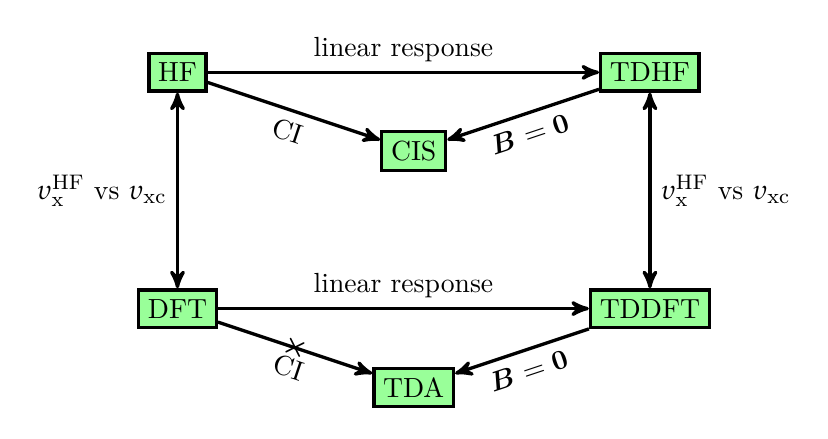
\begin{tikzpicture}
		\usetikzlibrary{shapes.misc}
		\begin{scope}[very thick,
			node distance=3cm,on grid,>=stealth',
			box/.style={rectangle,draw,fill=green!40}],
			\node [box, align=center]		(CIS)					{\textbf{CIS}};
			\node [box, align=center]		(HF)		[left=of CIS, yshift=1cm]	{\textbf{HF}};
			\node [box, align=center]		(TDHF)	[right=of CIS, yshift=1cm]	{\textbf{TDHF}};
			\node [box, align=center]		(DFT)	[below=of HF]	{\textbf{DFT}};
			\node [box, align=center]		(TDDFT)	[below=of TDHF]	{\textbf{TDDFT}};
			\node [box, align=center]		(TDA)	[below=of CIS]	{\textbf{TDA}};
			\path 
			(CIS) edge [<-]		node[below,sloped]{CI}									(HF)
			(CIS) edge [<-]		node[below,sloped]{$\bB{}{}=\bO$}								(TDHF)
			(HF) edge [->]		node[above]{linear response}								(TDHF)
			(HF) edge [<->]		node[left]{$\upsilon_\text{x}^\text{HF}$ vs $\upsilon_\text{xc}$}				(DFT)
			(TDHF) edge [<->]	node[right]{$\upsilon_\text{x}^\text{HF}$ vs $\upsilon_\text{xc}$}				(TDDFT)
			(DFT) edge [->]		node[above]{linear response}								(TDDFT)
			(DFT) edge [->]		node[below,sloped]{CI}	node[strike out,sloped]{\alert{$\cross$}}	(TDA)
			(TDDFT) edge [->]	node[below,sloped]{$\bB{}{}=\bO{}{}$}								(TDA)
			;
		\end{scope}
	\end{tikzpicture}
\end{frame}
%-----------------------------------------------------

%-----------------------------------------------------
\begin{frame}{Linear response}
	\begin{block}{General linear response problem}
		\begin{algorithmic}
			\Procedure{Linear response}{}
				\State Compute $\red{\bA{}{}}$ matrix at a given level of theory (RPA, RPAx, TD-DFT, BSE, etc)
				\If{$\TDA$} 
					\State Diagonalize $\red{\bA{}{}}$ to get $\highlight{\Om{m}{\TDA}}$ and $\bX{m}{\TDA}$
				\Else
					\State Compute \orange{$\bB{}{}$} matrix at a given level of theory
					\State Diagonalize $\red{\bA{}{}} - \orange{\bB{}{}}$ to form $(\red{\bA{}{}} - \orange{\bB{}{}})^{1/2}$
					\State Form and diagonalize $(\red{\bA{}{}} - \orange{\bB{}{}})^{1/2} \cdot (\red{\bA{}{}} + \orange{\bB{}{}}) \cdot (\red{\bA{}{}} - \orange{\bB{}{}})^{1/2}$ 
					to get $\highlight{\Om{m}{2}}$ and $\bZ{m}{}$
					\State Compute $\sqrt{\highlight{\Om{m}{2}}}$ and $(\bX{m}{} + \bY{m}{}) = \highlight{\Om{m}{-1/2}} (\red{\bA{}{}} - \orange{\bB{}{}})^{1/2} \cdot \bZ{m}{}$
				\EndIf
			\EndProcedure
		\end{algorithmic}
	\end{block}
\end{frame}
%-----------------------------------------------------

%-----------------------------------------------------
\begin{frame}{Form linear response matrices}
	\begin{block}{Linear-response matrices for BSE}
		\begin{algorithmic}
			\Procedure{Form $\red{\bA{}{}}$ for singlet states}{}
				\State Set $\red{\bA{}{}} = \bO$
				\State $ia \gets 0$ 
				\For{$i=1, \ldots, O$}
					\For{$a=1, \ldots, V$}
						\State $ia \gets ia + 1$
						\State $jb \gets 0$ 
						\For{$j=1, \ldots, O$}
							\For{$b=1, \ldots, V$}
								\State $jb \gets jb + 1$
								\State $\red{A_{ia,jb}} = \delta_{ij} \delta_{ab} (\e{a}{\green{GW}} - \e{i}{\green{GW}}) 
								+ 2\blue{(ia|bj)} - \yellow{(ij|ba)} + \purple{W^{\co}_{ij,ba}}(\omega = 0)$
							\EndFor 
						\EndFor 
					\EndFor 
				\EndFor 
			\EndProcedure
		\end{algorithmic}
	\end{block}
\end{frame}
%-----------------------------------------------------


%-----------------------------------------------------
\begin{frame}{Properties}
	\begin{block}{Oscillator strength (length gauge)}
		\begin{equation}
			\boxed{\green{f_m} = \frac{2}{3} \orange{\Om{m}{}} \qty[ (\blue{\mu_m^x})^2 + (\blue{\mu_m^y})^2 + (\blue{\mu_m^z})^2 ]}
		\end{equation}
	\end{block}
	\begin{block}{Transition dipole}
		\begin{equation}
			\boxed{\blue{\mu_m^x} = \sum_{ia} \red{(i|x|a)} \orange{(\bX{m}{} + \bY{m}{})_{ia}}}
			\qquad
			\red{(p|x|q)} = \int \MO{p}(\br) \,x\, \MO{q}(\br) d\br
		\end{equation}
	\end{block}
	\begin{block}{Monitoring possible spin contamination \pub{[Monino \& Loos, JCTC 17 (2021) 2852]}}
		\begin{equation}
			\boxed{\purple{\expval{\hat{S}^2}_m} = \violet{\expval{\hat{S}^2}_0} + \underbrace{\Delta \expval{\hat{S}^2}_m}_{\text{\pub{JCP 134101 (2011) 134}}}}
			\qquad
			\violet{\expval{\hat{S}^2}_0} = \frac{n_\alpha - n_\beta}{2} \qty( \frac{n_\alpha - n_\beta}{2} + 1 ) + n_\beta + \sum_p (p_\alpha|p_\beta)
		\end{equation}
	\end{block}
\end{frame}
%-----------------------------------------------------


%-----------------------------------------------------
\begin{frame}{Example from \texttt{QuAcK} (\ce{H2O}/cc-pVDZ)}
	\begin{center}
		\includegraphics[height=0.45\textwidth]{fig/BSE1}
		\hspace{0.05\textwidth}
		\includegraphics[height=0.45\textwidth]{fig/BSE3}
		\\
		\bigskip
		\pub{https://github.com/pfloos/QuAcK}
	\end{center}
\end{frame}
%-----------------------------------------------------

%-----------------------------------------------------
\begin{frame}{Open-shell systems and double excitations}
	\begin{block}{Spin-flip formalism  (H2/cc-pVQZ)}
		\begin{center}
			\includegraphics[width=0.28\textwidth]{fig/SFBSE}
			\includegraphics[width=0.4\textwidth]{fig/H2}
			\includegraphics[width=0.3\textwidth]{fig/H2_QuAcK}
			\\
			\bigskip
			\pub{Monino \& Loos, JCTC 17 (2021) 2852}
		\end{center}
	\end{block}
\end{frame}
%-----------------------------------------------------

%-----------------------------------------------------
\section{Correlation energy}
\begin{frame}
\tableofcontents[currentsection]
\end{frame}
%-----------------------------------------------------
\begin{frame}{Correlation energy at the $GW$ or BSE level}
	\begin{block}{RPA@$GW$ correlation energy: plasmon (or trace) formula}
		\begin{equation*}
			\label{eq:Ec-RPA}
			\green{\EcRPA} 
			= \frac{1}{2} \qty[ \sum_{p} \orange{\Om{m}{\RPA}} - \Tr(\orange{\bA{}{\RPA}}) ]
			= \frac{1}{2} \sum_{m} \qty( \orange{\Om{m}{\RPA}} - \orange{\Om{m}{\TDA}} )
		\end{equation*}
	\end{block}
	\begin{block}{Galitskii-Migdal functional}
		\begin{equation*}
			\label{eq:GM}
			\green{\EcGM} 
			= \frac{-i}{2}\sum_{pq}^{\infty}\int \frac{d\omega}{2\pi} \red{\SigC{pq}}(\omega) \blue{\G{pq}}(\omega) e^{i\omega\eta}
			= 4 \sum_{ia} \sum_{m} \frac{\violet{\ERI{ai}{m}}^2}{\blue{\eGW{a}} - \blue{\eGW{i}} + \orange{\Om{m}{\RPA}}}
		\end{equation*}
	\end{block}
	\begin{block}{ACFDT@BSE@$GW$ correlation energy from the adiabatic connection}
		\begin{equation}
			\green{\Ec^\text{ACFDT}} = \frac{1}{2} \int_{\red{0}}^{\red{1}} \Tr( \bK{}{} \bP{}{\la}) d\la
		\end{equation}
	\end{block}

\end{frame}
%-----------------------------------------------------

%-----------------------------------------------------
\begin{frame}{Adiabatic connection fluctuation dissipation theorem (ACFDT)}
	\begin{block}{Adiabatic connection}
		\begin{equation}
			\boxed{
				\green{\Ec^\text{ACFDT}}
				= \frac{1}{2} \int_{\red{0}}^{\red{1}} \Tr( \bK{}{} \bP{}{\la}) d\la
				\stackrel{\blue{\text{quad}}}{\approx} \frac{1}{2} \sum_{k=1}^{K} \purple{w_k} \Tr( \bK{}{} \bP{}{\violet{\lambda_k}}) 
			}
		\end{equation}
		$\la$ is the \textbf{strength} of the electron-electron interaction:
			\begin{itemize}
				\item $\la = 0$ for the \green{non-interacting system}
				\item $\la = 1$ for the \alert{physical system}
			\end{itemize}
	\end{block}
	\begin{block}{Interaction kernel}
		\begin{equation}
			\bK{}{} = 
			\begin{pmatrix}
				\btA{}{} & \btB{}{}
				\\
				\btB{}{}  & \btA{}{}
			\end{pmatrix}
			\qquad
			\tA{ia,jb}{} =  2\ERI{ia}{bj}
			\qquad
			\tB{ia,jb}{} =  2\ERI{ia}{jb}
		\end{equation}
	\end{block}
	\begin{block}{Correlation part of the two-particle density matrix}
		\begin{equation}
			\bP{}{\la} = 
			\begin{pmatrix}
				\bY{}{\la} \cdot \T{(\bY{}{\la})} & \bY{}{\la} \cdot \T{(\bX{}{\la})}
				\\
				\bX{}{\la} \cdot \T{(\bY{}{\la})}  & \bX{}{\la} \cdot \T{(\bX{}{\la})}
			\end{pmatrix}
			-
			\begin{pmatrix}
				\bO & \bO
				\\
				\bO  & \bI
			\end{pmatrix}
		\end{equation}
	\end{block}
\end{frame}
%-----------------------------------------------------

%-----------------------------------------------------
\begin{frame}{Gaussian quadrature}
	\begin{block}{Numerical integration by quadrature}
		\textit{``A $K$-point \orange{Gaussian quadrature} rule is a quadrature rule constructed to yield an exact result for polynomials up to degree $2K-1$ by a suitable choice of the \violet{roots $x_k$} and \purple{weights $w_k$} for $k = 1, \ldots, K$.''}
		\begin{equation}
			\boxed{\int_{\red{a}}^{\red{b}} f(x) \purple{w(x)} dx \approx \sum_k^{K} \underbrace{\purple{w_k}}_{\text{\purple{weights}}} f(\underbrace{\violet{x_k}}_{\text{\violet{roots}}})}
		\end{equation}
	\end{block}
	\begin{block}{Quadrature rules}
		\begin{center}
			\small
			\begin{tabular}{llll}
				\hline
				\red{Interval $[a,b]$}	&	\purple{Weight function $w(x)$}					&	\violet{Orthogonal polynomials}			&	\orange{Name}	\\
				\hline
				$[-1,1]$			&	$1$													&	Legendre $P_n(x)$						&	Gauss-Legendre	\\
				$(-1,1)$			&	$(1-x)^\alpha(1+x)^\beta, \quad \alpha,\beta > -1$	&	Jacobi $P_n^{\alpha,\beta}(x)$			&	Gauss-Jacobi	\\
				$(-1,1)$			&	$1/\sqrt{1-x^2}$									&	Chebyshev (1st kind) $T_n(x)$			&	Gauss-Chebyshev	\\
				$[-1,1]$			&	$\sqrt{1-x^2}$										&	Chebyshev (2nd kind) $U_n(x)$			&	Gauss-Chebyshev	\\
				$[0,\infty)$		&	$\exp(-x)$											&	Laguerre $L_n(x)$ 						&	Gauss-Laguerre	\\
				$[0,\infty)$		&	$x^\alpha \exp(-x), \quad \alpha > -1$				&	Generalized Laguerre $L_n^\alpha(x)$	&	Gauss-Laguerre	\\
				$(-\infty,\infty)$	&	$\exp(-x^2)$										&	Hermite $H_n(x)$ 						&	Gauss-Hermite	\\
				\hline
			\end{tabular}
			 \\
			 \url{https://en.wikipedia.org/wiki/Gaussian_quadrature}
		\end{center}
	\end{block}
\end{frame}
%-----------------------------------------------------

%-----------------------------------------------------
\begin{frame}{ACFDT at the RPA/RPAx level}
	\begin{block}{RPA matrix elements}
		\begin{equation}
			\orange{\A{ia,jb}{\la,\RPA}} = \delta_{ij} \delta_{ab} (\violet{\eHF{a}} - \violet{\eHF{i}}) + 2\la\ERI{ia}{bj}
			\qquad 
			\orange{\B{ia,jb}{\la,\RPA}} = 2\la\ERI{ia}{jb}
		\end{equation}
		\begin{equation}
			\boxed{
				\green{\Ec^\RPA} 
				= \frac{1}{2} \int_{\red{0}}^{\red{1}} \Tr( \bK{}{} \bP{}{\la}) d\la
				= \frac{1}{2} \qty[ \sum_{m} \orange{\Om{m}{\RPA}} - \Tr(\orange{\bA{}{\RPA}}) ] 
			}
		\end{equation}
	\end{block}

	\begin{block}{RPAx matrix elements}
		\begin{equation}
			\orange{\A{ia,jb}{\la,\RPAx}} = \delta_{ij} \delta_{ab} (\violet{\eHF{a}} - \violet{\eHF{i}}) + \la \qty[2 \ERI{ia}{bj} - \ERI{ij}{ab} ]
			\qquad 
			\orange{\B{ia,jb}{\la,\RPAx}} = \la \qty[2 \ERI{ia}{jb} - \ERI{ib}{aj} ]
		\end{equation}
		\begin{equation}
			\boxed{
				\green{\Ec^\RPAx} 
				= \frac{1}{2} \int_{\red{0}}^{\red{1}} \Tr( \bK{}{} \bP{}{\la}) d\la
				\alert{\neq} \frac{1}{2} \qty[ \sum_{m} \orange{\Om{m}{\RPAx}} - \Tr(\orange{\bA{}{\RPAx}}) ] 
			}
		\end{equation}
		If exchange added to kernel, i.e., $\bK{}{} = \bK{}{\x}$, then \pub{[Angyan et al. JCTC 7 (2011) 3116]}
		\begin{equation}
			\green{\Ec^\RPAx} 
			= \frac{1}{4} \int_{\red{0}}^{\red{1}} \Tr( \bK{}{\x} \bP{}{\la}) d\la
			\alert{=} \frac{1}{4} \qty[ \sum_{m} \orange{\Om{m}{\RPAx}} - \Tr(\orange{\bA{}{\RPAx}}) ] 
		\end{equation}
	\end{block}
\end{frame}
%-----------------------------------------------------
	
	
%-----------------------------------------------------
\begin{frame}{ACFDT at the BSE level}
	\begin{block}{BSE matrix elements}
		\begin{equation}
			\orange{\A{ia,jb}{\la,\BSE}} = \delta_{ij} \delta_{ab} (\violet{\eGW{a}} - \violet{\eGW{i}}) + \la \qty[2 \ERI{ia}{bj} - \highlight{W}_{ij,ab}^{\la}(\omega = 0) ]
			\qquad 
			\orange{\B{ia,jb}{\la,\BSE}} = \la \qty[2 \ERI{ia}{jb} - \highlight{W}_{ib,ja}^{\la}(\omega = 0)]
		\end{equation}
		\begin{equation}
			\boxed{
				\green{\Ec^\BSE} 
				= \frac{1}{2} \int_{\red{0}}^{\red{1}} \Tr( \bK{}{} \bP{}{\la}) d\la
				\alert{\neq} \frac{1}{2} \qty[ \sum_{m} \orange{\Om{m}{\BSE}} - \Tr(\orange{\bA{}{\BSE}}) ] 
			}
		\end{equation}

	\end{block}
	\begin{block}{$\la$-dependent screening}
		\begin{equation}
			\highlight{W}_{pq,rs}^{\la}(\omega) 
			= \ERI{pq}{rs}
			+ 2 \sum_m \violet{\ERI{pq}{m}^{\la}} \violet{\ERI{rs}{m}^{\la}}
			\qty[ \frac{1}{\omega - \orange{\Om{m}{\la,\RPA}} + i \eta} - \frac{1}{\omega + \orange{\Om{m}{\la,\RPA}} - i \eta} ]
		\end{equation}
		\begin{equation}
			\violet{\ERI{pq}{m}^{\la}} = \sum_{ia} \ERI{pq}{ia} (\orange{\bX{m}{\la,\RPA}+\bY{m}{\la,\RPA}})_{ia}
		\end{equation}
	\end{block}
\end{frame}
%-----------------------------------------------------

%-----------------------------------------------------
\begin{frame}{ACFDT in a computer}
	\begin{block}{ACFDT correlation energy from BSE}
		\begin{algorithmic}
			\Procedure{ACFDT for BSE}{}
				\State Compute $GW$ quasiparticle energies $\blue{\beGW}$ and interaction kernel $\bK{}{}$
				\State Get Gauss-Legendre weights and roots $\{\purple{w_k},\violet{\lambda_k}\}_{1\le k \le K}$
				\State $\green{\Ec} \gets 0$
				\For{$k=1,\ldots,K$}
					\State Compute static screening elements $\highlight{W}_{pq,rs}^{\violet{\lambda_k}}(\omega = 0)$ 
					\State Perform BSE calculation at $\la = \violet{\lambda_k}$ to get $\bX{}{\violet{\lambda_k}}$ and $\bY{}{\violet{\lambda_k}}$
					\Comment{\alert{This is a $\order*{N^6}$ step done many times!}}
					\State Form two-particle density matrix $\bP{}{\violet{\lambda_k}}$
					\State $\green{\Ec} \gets \green{\Ec} + \purple{w_k} \Tr( \bK{}{} \bP{}{\violet{\lambda_k}})$
				\EndFor
			\EndProcedure
		\end{algorithmic}
	\end{block}
\end{frame}
%-----------------------------------------------------

%-----------------------------------------------------
\begin{frame}
	\begin{center}
		\includegraphics[width=0.7\textwidth]{fig/TOC_BSE}
		\\
		\pub{Loos et al. JPCL 11 (2020) 3536}
	\end{center}
\end{frame}
%-----------------------------------------------------

%-----------------------------------------------------
\begin{frame}{Useful papers/programs}
	\begin{itemize}
		\item \red{mol$GW$:} Bruneval et al. Comp. Phys. Comm. 208 (2016) 149
		\bigskip
		\item \green{Turbomole:} van Setten et al. JCTC 9 (2013) 232; Kaplan et al. JCTC 12 (2016) 2528
		\bigskip
		\item \violet{Fiesta:} Blase et al. Chem. Soc. Rev. 47 (2018) 1022
		\bigskip
		\item \purple{FHI-AIMS:} Caruso et al. PRB 86 (2012) 081102
		\bigskip
		\item \orange{Reviews \& Books:} 
			\begin{itemize}
				\item Reining, WIREs Comput Mol Sci 2017, e1344. doi: 10.1002/wcms.1344
				\item Onida et al. Rev. Mod. Phys. 74 (2002) 601
				\item Blase et al. Chem. Soc. Rev. , 47 (2018) 1022
				\item Golze et al. Front. Chem. 7 (2019) 377
				\item Blase et al. JPCL 11 (2020) 7371
				\item Martin, Reining \& Ceperley \textit{Interacting Electrons} (Cambridge University Press)
			\end{itemize}
		\bigskip
		\item \red{$GW$100:} IPs for a set of 100 molecules. van Setten et al. JCTC 11 (2015) 5665 (\url{http://gw100.wordpress.com})
		
	\end{itemize}
\end{frame}
%-----------------------------------------------------

\end{document}
